 \chapter{La détection d'objets}
\minitoc
\newpage
\pagestyle{fancy}
\fancyhead[L]{\chaptername \ \thechapter}
\fancyhead[R]{La détection d'objets}
\renewcommand{\headrulewidth}{1pt}
\fancyfoot[C]{\thepage}

\section{Introduction} 
La détection d'objet est un sous-domaine de vision par ordinateur dont le but de localiser la position de l'objet recherché et d'identifier en lui attribuant la classe appropriée dans une image numérique. Le besoin de détection d'objets est d'automatiser les tâches difficiles qui nécessitent une intervention humaine ou impossible à faire par l'homme. Par exemple, la tâche de lire le numéro d'immatriculation
de chaque voiture qui passe sur l'autoroute où les voitures passent à grande vitesse que l'œil humain avec le cerveau est incapable de percevoir quelques chiffres, sans parler du numéro d'enregistrement complet.
\section{Objectif}
L'objectif de la détection d'objets est divisé en 2 composants principaux; premièrement, la localisation d'objets et deuxièmement, l'identification ou la classification d'objets.
\subsection{Localisation d'objet}
Ce composant est la principale différence entre la détection d'objet dans l'image et la classification d'image où, dans la classification d'image, l'objet est identifié uniquement sans son emplacement dans l'image, d'autre part, dans la détection d'objet, l'objet est également localisé en utilisant la technique de la boîte englobante ou technique basée sur les pixels qui se divise également en segmentation sémantique et segmentation d'instance.
\subsubsection{Boîte englobante (Bounding Box)}
La technique de la boîte englobante est la méthode traditionnelle d'étiquetage des données dans l'image. Les cadres de délimitation sont des marqueurs d'annotation dessinés autour des objets dans une image. Contours mais en forme de forme rectangulaire. Il a fait l'objet des études les plus approfondies en raison de sa facilité d'utilisation et de calcul.

\begin{figure}[H]
\centering
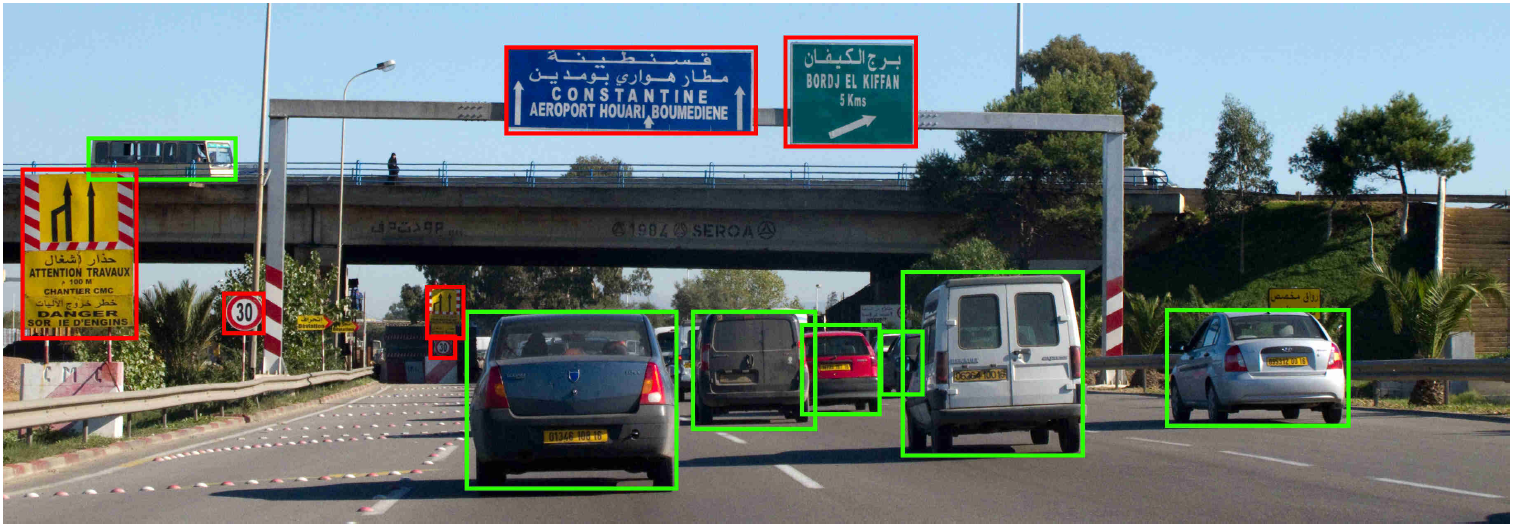
\includegraphics[height=5.7cm,width=16cm]{Chapitre1/im4.png}
\caption{---------.}
\label{im4}
\end{figure}

\subsubsection{Mask (niveau de pixel)}
La deuxième technique utilisée dans la détection d'objets est basée sur les pixels. il nécessite de segmenter l'objet en pixel au lieu de la boîte englobante. cette technique donne un emplacement précis (au niveau du pixel) d'un objet et des pixels trouvés. les pixels produits peuvent aussi être appelés le masque. Il existe 2 types de segmentation, la premier est la segmentation sémantique où tous les objets de la même classe obtiennent le même pixel, où dans le deuxième type, la segmentation d'instance, chaque objet de l'image obtient son masque unique même s'il existe d'autres objets avec la même classe. En raison de la nature de bas niveau de cette technique, elle nécessite une puissance de calcul importante pour segmenter l'objet pixel par pixel, de plus cette technique est assez nouvelle et encore immature en raison des faibles études appliquées dans celle-ci.

\begin{figure}[H]
\centering
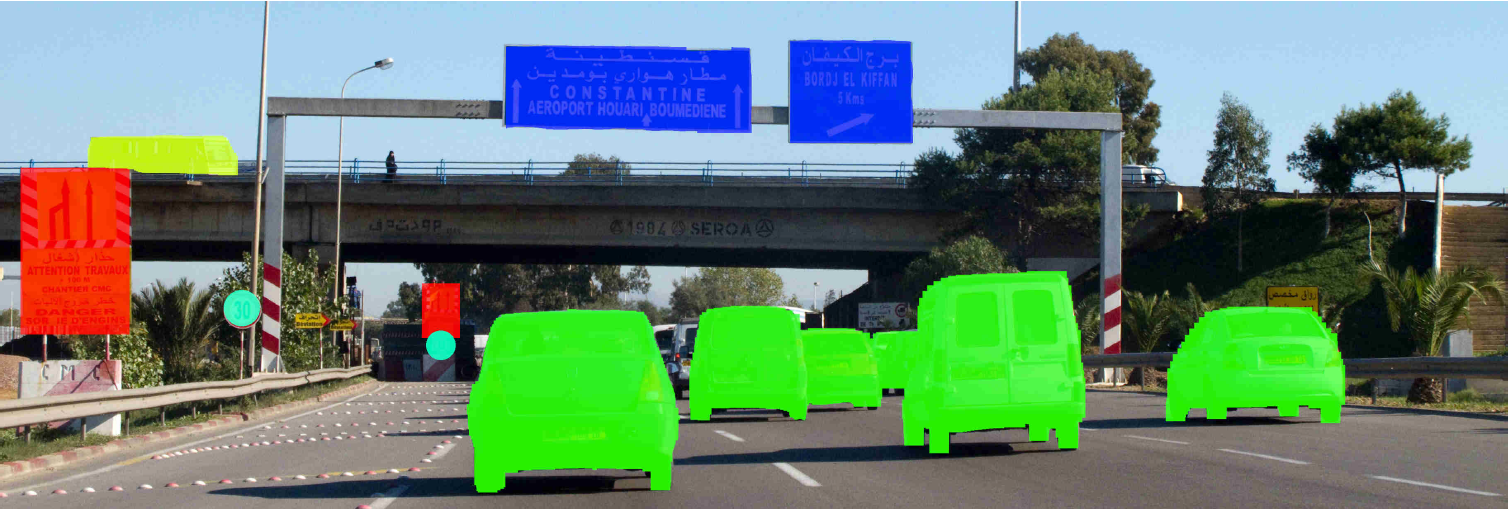
\includegraphics[height=5.7cm,width=16cm]{Chapitre1/im5.png}
\caption{---------.}
\label{im5}
\end{figure}
\begin{figure}[H]
\centering
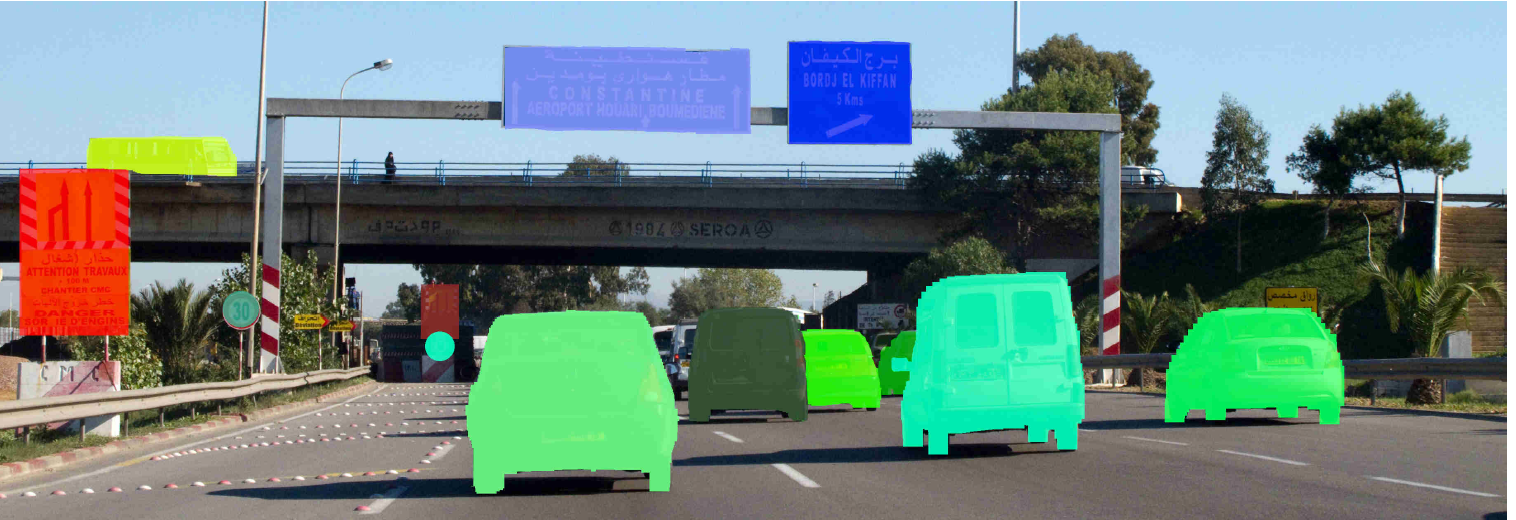
\includegraphics[height=5.7cm,width=16cm]{Chapitre1/im6.png}
\caption{---------.}
\label{im6}
\end{figure}


\subsection{Classification d'objet}
Le deuxième composant est la reconnaissance d'objets. La reconnaissance est la capacité du modèle (le réseau de neurones dans notre cas) à identifier un objet en fonction de certaines similitudes qu'il partage avec un autre objet que le modèle a déjà rencontré. La reconnaissance peut être basée sur une inférence ou une relation, c'est-à-dire une situation dans laquelle un modèle est capable de reconnaître un objet parce qu'il reconnaît les similitudes de
forme et de propriétés. La reconnaissance peut également se produire parce que le modèle a rencontré l'objet exact lors d'une instance précédente Chez les êtres humains, la reconnaissance est un processus cognitif qui se déroule de manière transparente et presque instantanément sans délai. Le cerveau humain est capable d'apprendre et d'adapter des informations avec un minimum d'effort, de sorte que même les humains qui en sont encore aux stades de développement de leur existence peuvent facilement reconnaître les objets. Les humains peuvent reconnaître une multitude d'objets dans des images avec peu d'effort, même si l'image des objets peut varier quelque peu selon différents points de vue, dans de nombreuses tailles et échelles
différentes ou même lorsqu'ils sont déplacés ou pivotés. Les objets peuvent même être reconnus lorsqu'ils sont partiellement masqués. La machine ou le modèle, cependant, ne possède pas de façon innée cette capacité cognitive.
Pour que l'intelligence artificielle acquière ce niveau de compétence, elle doit acquérir une formation. Cette formation est généralement acquise en apprenant les jeux de données du modèle. Cette tâche reste un défi pour les systèmes de vision par ordinateur étant donné que ces modèles doivent être entraînés pour chaque classe d'objets qu'ils sont censés reconnaître.

\begin{figure}[H]
\centering
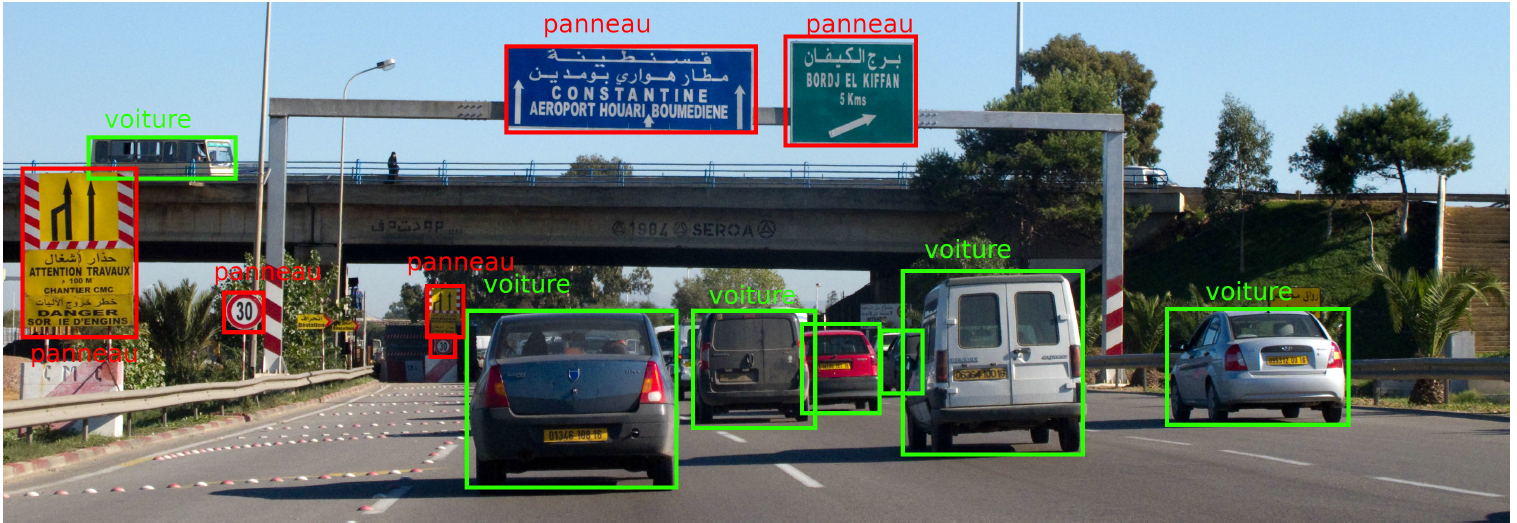
\includegraphics[height=6cm,width=16cm]{Chapitre1/im7.png}
\caption{---------.}
\label{im7}
\end{figure}

\section{Historique}
L'histoire de la détection d'objets est divisée en 2 époques la première époque est nommée l'époque traditionnelle ou l'époque avant l'apprentissage profond où les ressources étaient extrêmement limitées qui incluent la faible puissance de calcul des machines avec le manque de représentation d'image efficace, par conséquent, les algorithmes qui ont été construits à cette époque sont basés sur des caractéristiques sélectionnées manuellement, comme les détecteurs Viola Jones développé par Paul Viola and Michael Jones en 2001
qui permis la détection de visages humains en temps réel à l'aide d'une fenêtre coulissante qui recherche les caractéristiques du visage, malheureusement, la détection d'objets a atteint un plateau après 2010, car les performances des caractéristiques sélectionnées manuellement sont devenues saturées.
Après la généralisation d'Internet dans le monde entier et l'augmentation des données flottant sur le Web qui ont conduit à la création d'ImageNet, une grande base de données visuelle conçue pour être utilisée dans la recherche de logiciels de reconnaissance visuelle d'objets. et l'augmentation drastique de la puissance de calcul des machines provoquée par le développement de systèmes de calcul parallèles comme les super-machines de calcul haute performance (HPC), A ouvert la voie à l'apprentissage profond en particulier aux réseaux de neurones convolutifs (CNN) A ouvert la voie à l'apprentissage en profondeur, en particulier aux réseaux de neurones
convolutifs et le plus célèbre est AlexNet implementé par Alex Krizhevsky en 2012. De nombreux algorithmes sont apparus après pour amélioré les performances et le résultat et nous utiliserons l'algorithme YOLO plus tard.
\section{Etat de l'art des techniques de détection d'objets}

----

 
\section{Les applications de la détection d'objets}
La détection d'objets fait son entrée dans un large éventail d'industries, avec des cas d'utilisation allant de la sécurité personnelle à la productivité sur le lieu de travail. La détection et la reconnaissance d'objets sont appliquées dans de nombreux domaines de la vision par ordinateur, notamment la récupération d'images, la sécurité, la surveillance, les systèmes de véhicules automatisés et l'inspection des machines. Des défis importants subsistent dans le domaine de la reconnaissance d'objets. Les possibilités sont infinies en ce qui concerne les futurs cas d'utilisation de la détection d'objets. Dans cette section, nous discutons  certaines applications actuelles et futures  des systèmes de détection d'objets dans divers domaines..
\subsection{Reconnaissance optique de caractères}

\subsection{Voitures autonomes}

\subsection{Suivi des objets}
Le système de détection d'objets est également utilisé pour suivre les objets, par exemple suivre un ballon pendant un match de football, suivre une personne dans une vidéo. Le suivi d'objets a une variété d'utilisations, dont certaines sont la surveillance et la sécurité , surveillance du trafic, communication vidéo, vision et animation de robots.

\begin{figure}[H]
\centering
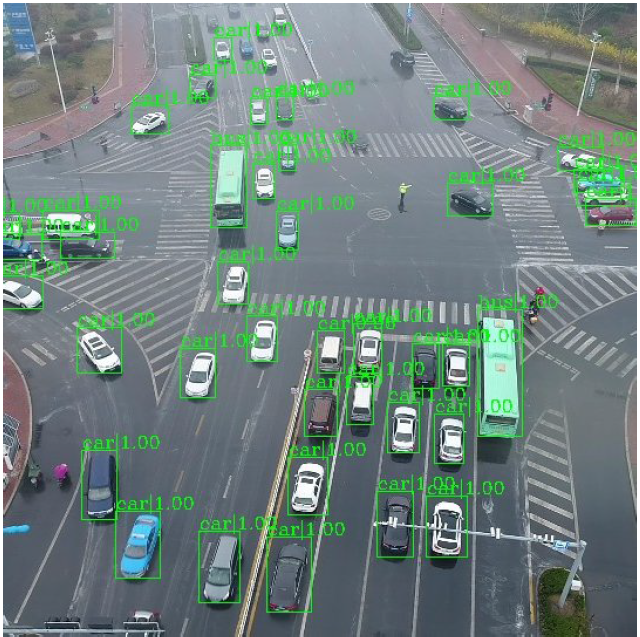
\includegraphics[height=6.5cm,width=6.5cm]{Chapitre1/im10.png}
\caption{---------.}
\label{im10}
\end{figure}

\subsection{Biométrie}

\subsection{reconnaissance d'activités}

\subsection{Tatouage numérique}

\subsection{Imagerie médicale}

\subsection{Robotique}

\subsection{Production industrielle}
Les usines du monde entier s'efforcent de produire des produits de la
meilleure qualité avec un coût de production minimum. Cependant, pour
atteindre cet objectif, les usines doivent embaucher de la main-d'œuvre pour vérifier la qualité des composants, ce qui augmente le coût de production et d'autres problèmes liés au travail manuel. comme la dextérité et la productivité du travailleur. La détection d'objets résout les problèmes liés au travail manuel. il garantit que les bons composants sont utilisés dans les chaînes de montage et que les processus corrects sont suivis avec une précision et une exactitude élevées, plus qu'un travailleur manuel et à moindre coût.

\begin{figure}[H]
\centering
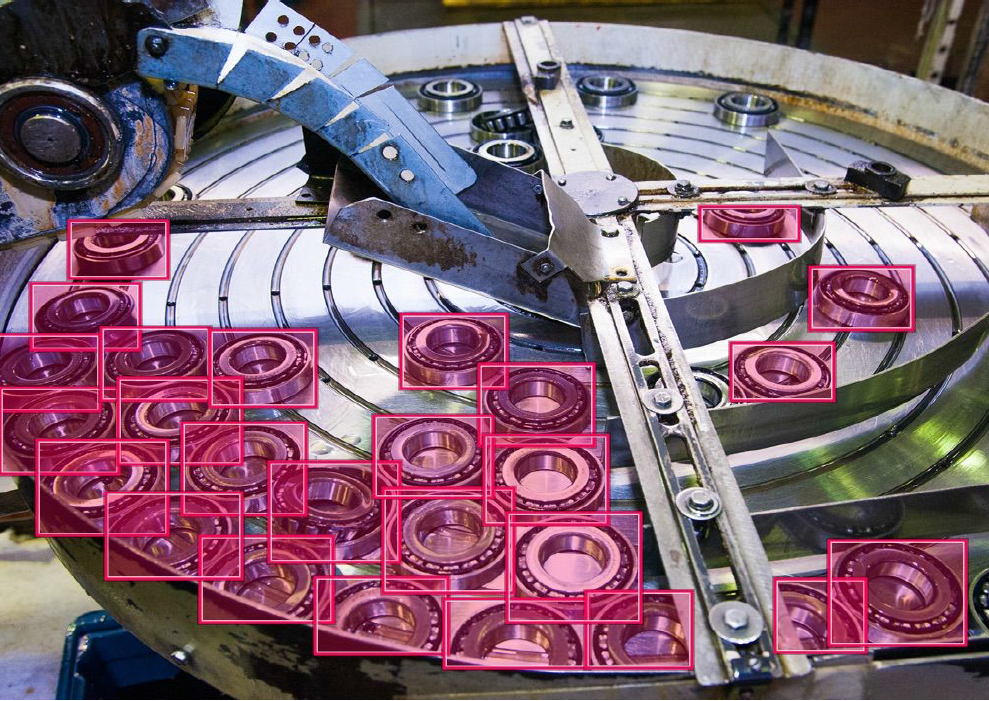
\includegraphics[height=7cm,width=12cm]{Chapitre1/im8.png}
\caption{---------.}
\label{im8}
\end{figure}

\subsection{Surveillance et sécurité}
Dans les grandes villes où la population est très élevée, dans les zones industrielles, les grandes banques et de nombreuses autres zones hautement sensibles, la sécurité est indispensable 24 heures sur 24 et il est presque impossible pour un être humain d'atteindre ce niveau. La détection d'objets est donc une solution à ce type de problèmes où elle suit les mouvements des visiteurs, suit les comportements des individus ou des véhicules, fait la distinction entre les activités autorisées et non autorisées et signale lorsqu'un objet inattendu nécessite une enquête. tout cela 24 heures sur 24 sans arrêt et
aussi à moindre coût de maintenance.

\begin{figure}[H]
\centering
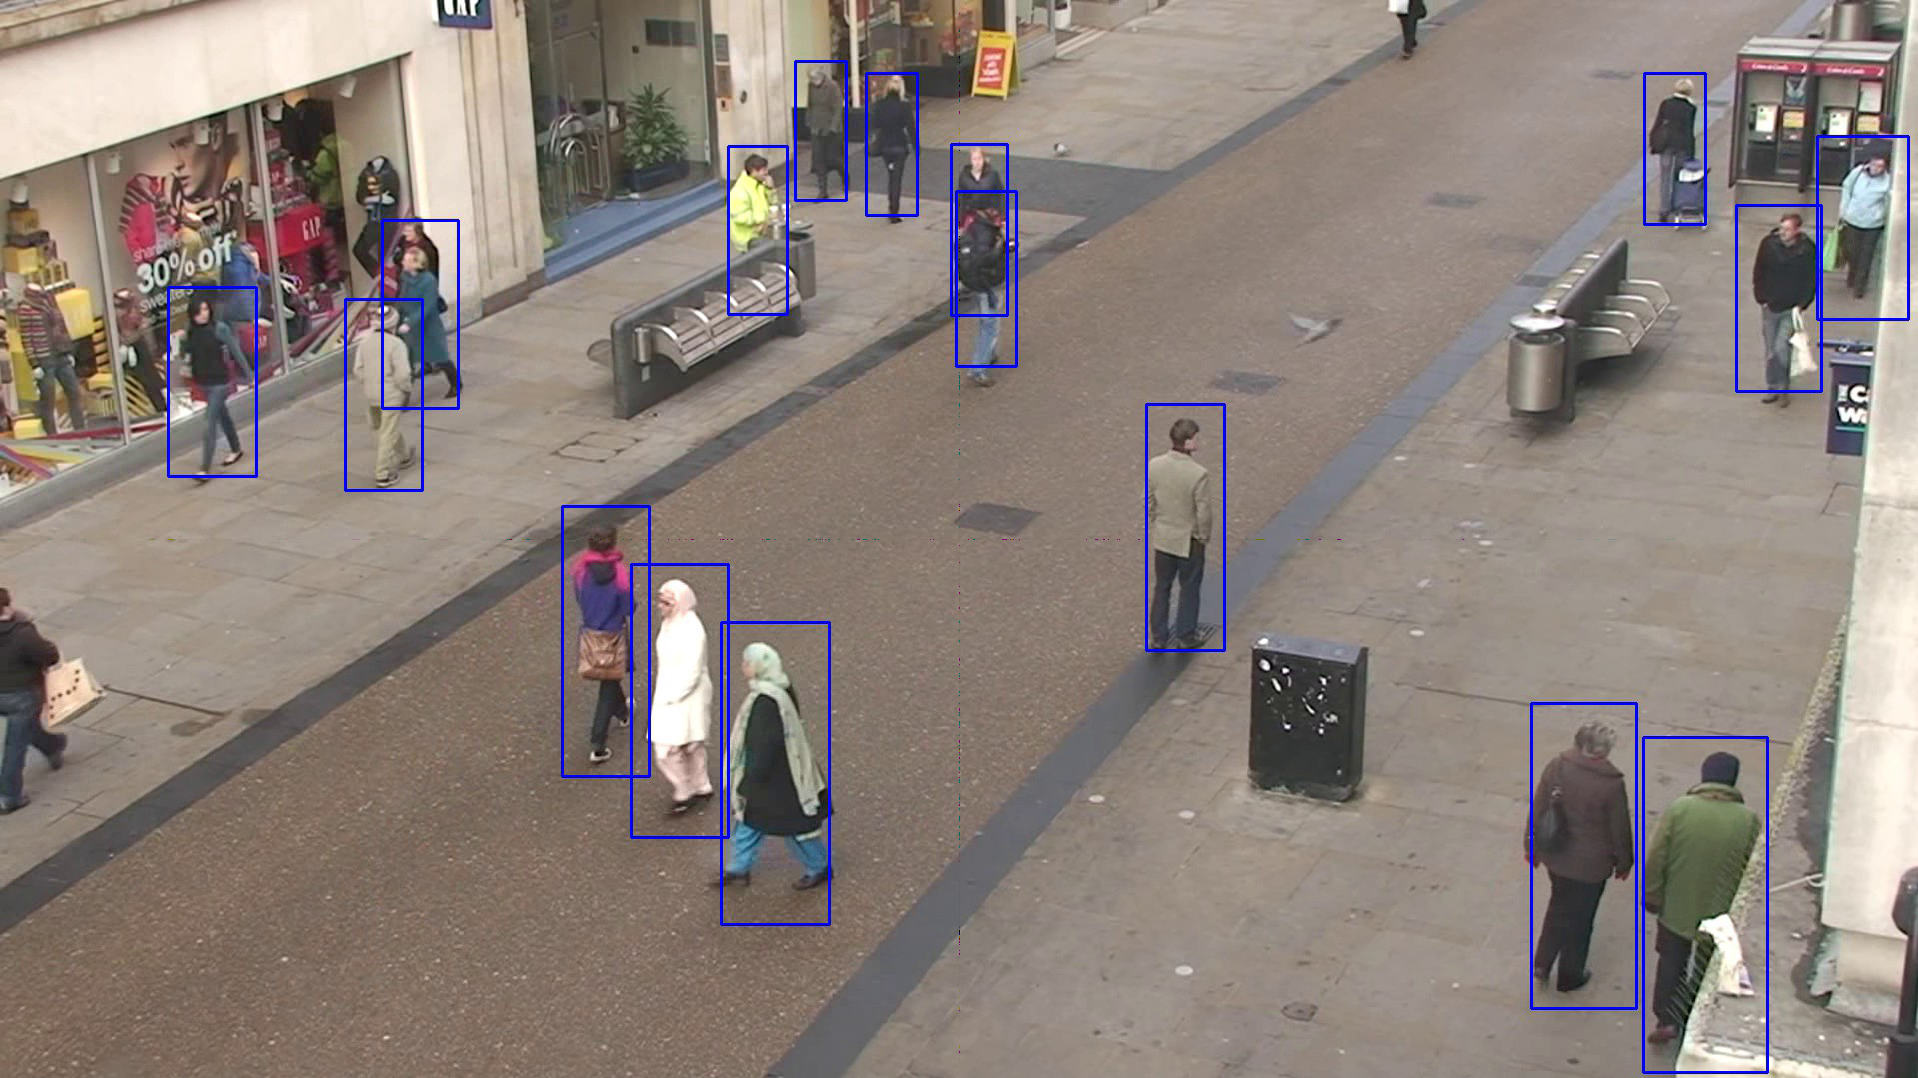
\includegraphics[height=6cm,width=14cm]{Chapitre1/im9.png}
\caption{---------.}
\label{im9}
\end{figure}

\section{Conclusion}

